\section{$n$-step Bootstrapping}
\subsection{Exercise 7.1}
\subsubsection{Q}
In Chapter 6 we noted that the Monte Carlo error can be written as the sum of TD errors (6.6) if the value estimates don’t change from step to step. Show that the n-step error used in (7.2) can also be written as a sum TD errors (again if the value estimates don’t change) generalizing the earlier result.
\subsubsection{A}
The $n$-step error in equation 7.2 is $G_{t:t+n} - V_{t+n-1}(S_t)$ and our generalised TD error is $\delta_{t:t+n} = R_{t+n+1} + \gamma V_{t+n}(S_{t+1}) - V_{t+n}(S_t)$. As in 6.6, we can rewrite this as:

\begin{align}
G_{t:t+n} - V_{t+n-1}(S_t) &= R_{t+n+1} + \gamma G_{t+n+1} - V_{t+n}(S_t) \\
&= R_{t+n+1} + \gamma G_{t+n+1} - V_{t+n}(S_t) + \gamma V_{t+n}(S_{t+1}) - \gamma V_{t+n}(S_{t+1}) \\
&= \delta_{t:t+n} + \gamma (G_{t+n+1} + V_{t+n}(S_{t+1})) \\
&= \delta_{t:t+n} + \gamma \left[R_{t+n+2} + \gamma G_{t+n+2} - V_{t+n+1}(S_{t+2})\right] \\
&= \delta_{t:t+n} + \gamma \delta_{t+1:t+n+1} + \gamma^2 (G_{t+n+2} + V_{t+n+1}(S_{t+1})) \\
&= \delta_{t:t+n} + \gamma \delta_{t+1:t+n+1} + \gamma^2 \delta_{t+2:t+n+2} + \cdots + \gamma^{T-t-1}(G_{t+n+T-t -1} - V_{t+n+T-t-2}(S_T) +  \gamma^{T-t}(G_{t+n+T-t} - V_{t+n+T-t-1}(S_T) \\
&= \delta_{t:t+n} + \gamma \delta_{t+1:t+n+1} + \gamma^2 \delta_{t+2:t+n+2} + \cdots + \gamma^{T-t-1}(G_{T+n-1} - V_{T+n-2}(S_T) +  \gamma^{T-t}(0) \\
&= \sum_{k=t}^{T-1} \gamma^{k-t} \delta_{t+k:n+k}\\
\end{align}
$
\hfill \blacksquare
$

\subsection{Exercise 7.2}
\subsubsection{Q}
With an $n$-step method, the value estimates do change from step to step, so an algorithm that used the sum of TD errors (see previous exercise) in place of the error in (7.2) would actually be a slightly different algorithm. Would it be a better algorithm or a worse one? Devise and program a small experiment to answer this question empirically.
\subsubsection{A}
\ProgrammingExercise \\

$
\hfill \blacksquare
$

\subsection{Exercise 7.3}
\subsubsection{Q}
Why do you think a larger random walk task (19 states instead of 5) was used in the examples of this chapter? Would a smaller walk have shifted the advantage to a different value of n? How about the change in left-side outcome from 0 to -1 made in the larger walk? Do you think that made any difference in the best value of n?
\subsubsection{A}
\begin{itemize}
	\item If the smaller, 5-state random walk had been used the optimal value for $n$ would likely have been smaller. As explained in the example, setting $n$ to 3 and observing an episode starting at $C$ and transitioning $C \rightarrow D \rightarrow E \rightarrow Terminal$ would update $C$ toward the reward of 1, which would represent an incorrect estimation of the true value of $C$. It seems that the likely optimal value in this case would be $n = 2$, and so we could make the general assumption that for smaller state-spaces, smaller values of $n$ are more appropriate. If $n \geq 2$ then, for longer episodes, updates would no longer be bootstrapping on other state value, but instead be making updates based on their own values.
	\item I suspect that the change in the left value to -1 from 0 reduced the optimal value of $n$ in this example. Setting the left value to -1 effectively locates states on the left side of the walk closer to a reward, meaning updates need not back-propagate as far to make good updates to the value of these states. 
\end{itemize}

$
\hfill \blacksquare
$

\subsection{Exercise 7.4}
\subsubsection{Q}
Prove that the $n$-step return of Sarsa (7.4) can be written exactly in terms of a novel TD error, as:
\begin{equation}
G_{t:t+n} = Q_{t-1}(S_t, A_t) + \sum_{k=t}^{min(t+n, T)-1} \gamma^{k-t}\left[R_{k+1} + \gamma Q_k(S_{k+1}, A_{k+1}) - Q_{k-1}(S_k, A_k) \right]
\end{equation}
\subsubsection{A}
We have:
\begin{equation}
G_{t:t+n} = R_{t+1} + \gamma R_{t+2} + \cdots + \gamma^{n-1}R_{t+n} + \gamma^n Q_{t+n-1}(S_{t+n}, A_{t+n})
\end{equation}
and:
\begin{equation}
Q_{t+n}(S_t, A_t) = Q_{t+n-1}(S_t, A_t) + \alpha \left[G_{t:t+n} - Q_{t+n-1}(S_t, A_t)\right]
\end{equation}

Denote:
\begin{equation}
G_{t:t+n} \doteq \sum_{i=1}^{n} \gamma^{i-1} R_{t+i} + \gamma^n Q_{t+n-1}(S_{t+n}, A_{t+n})
\end{equation}
for $n \geq 1$ and $0 \leq t < T - n$ and with $G_{t:t+n} = G_t$ if $t+n > T$

If we set $\tau = \min (t+n, T) - 1$, we observe that:
\begin{align}
\sum_{k=t}^{min(t+n, T)-1} \gamma^{k-t}\left[R_{k+1} + \gamma Q_k(S_{k+1}, A_{k+1}) - Q_{k-1}(S_k, A_k) \right] &= \sum_{k=t}^{\tau}\gamma^{k-t}\left[R_{t+1} + \gamma Q_k(S_{k+1}, A_{k+1} - Q_{k-1}(S_k, A_k)\right] \\
&= G_{t:t+n} - Q_{t-1}(S_t, A_t) \\
\end{align}

$
\hfill \blacksquare
$

\subsection{Exercise 7.5}
\subsubsection{Q}
Write the pseudocode for the off-policy state-value prediction algorithm described above.
\subsubsection{A}
The algorithm follows much the same form as that described on page 149:
\begin{figure}[h!]
	\centering
	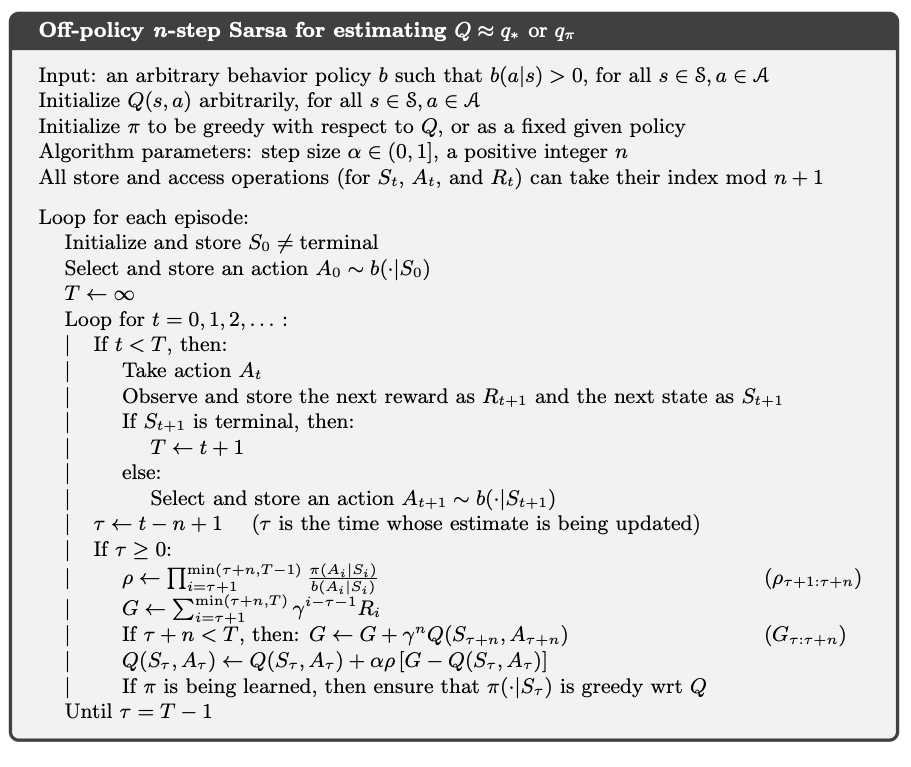
\includegraphics[width=\textwidth]{/ex7.5}
	\caption{Off-policy n-step sarsa pseudocode}
	\label{fig: n-step sarsa methods}
\end{figure}

Of course, this time we initialize $V(s)$ arbitrarily instead of $Q(s,a)$. In the final if statement, $G$ instead becomes:
\begin{equation}
G \leftarrow \rho_\tau \left(R_{\tau+1} + \sum_{i = \tau + 1}^{min(\tau+n, T)} \gamma^{i - \tau -1} R_i\right) + (1 - \rho_\tau)V_{\tau+n-1}(S_t)
\end{equation}
and the state value update becomes:
\begin{equation}
V(S_\tau) \leftarrow V(S_\tau) + \alpha \left[G - V(S_\tau)\right]
\end{equation}

$
\hfill \blacksquare
$

\subsection{Exercise 7.6}
\subsubsection{Q}
Prove that the control variate in the above equations does not change the expected value of the return.
\subsubsection{A}
In equation 7.13, we know that the expected value of $\rho_t =1$, therefore:
\begin{align}
	\mathbb{E}\left[(1-\rho_t) V_{h-1}(S_t)\right] &= \mathbb{E}_b\left[(1-\rho_t) V_{h-1}(S_t)\right] \\
	&= \mathbb{E}_b\left[(1-\rho_t) V_{h-1}(S_t)\right] \\
	&= \mathbb{E}_b\left[(1-1) V_{h-1}(S_t)\right] \\
	&= 0\\
\end{align}
In equation 7.14, the control variate is slightly different, we have:
\begin{align}
	\mathbb{E}_b\left[\bar{V}_h-1(S_{t+1} - \rho_{t+1}Q_h-1(S_{t+1}, A_{t+1}))\right] &= \sum_{a} \pi(a | S_{t+1}) Q_{h-1}(S_{t+1}, a) - \sum_{a}b(a | S_{t+1}) \rho_{t+1} Q_{h-1}(S_{t+1}, a) \\
	&= \sum_{a} \pi(a | S_{t+1}) Q_{h-1}(S_{t+1}, a) - \sum_{a}b(a | S_{t+1}) \frac{\pi(a | S_{t+1})}{b(a | S_{t+1})} Q_{h-1}(S_{t+1}, a) \\
	&= 0 \\
\end{align}
$
\hfill \blacksquare
$

\subsection{Exercise 7.7}
\subsubsection{Q}
Write the pseudocode for the off-policy action-value prediction algorithm described immediately above. Pay particular attention to the termination conditions for the recursion upon hitting the horizon or the end of episode.
\subsubsection{A}
TBC

$
\hfill \blacksquare
$

\subsection{Exercise 7.8}
\subsubsection{Q}
Show that the general (off-policy) version of the n-step return (7.13) can still be written exactly and compactly as the sum of state-based TD errors (6.5) if the approximate state value function does not change.
\subsubsection{A}
TBC

$
\hfill \blacksquare
$

\subsection{Exercise 7.9}
\subsubsection{Q}
Repeat the above exercise for the action version of the off-policy n-step return (7.14) and the Expected Sarsa TD error (the quantity in brackets in Equation 6.9).
\subsubsection{A}
TBC

$
\hfill \blacksquare
$

\subsection{Exercise 7.10}
\subsubsection{Q}
Devise a small off-policy prediction problem and use it to show that the off-policy learning algorithm using (7.13) and (7.2) is more data efficient than the simpler algorithm using (7.1) and (7.9).
\subsubsection{A}
TBC

$
\hfill \blacksquare
$

\subsection{Exercise 7.11}
\subsubsection{Q}
Show that if the approximate action values are unchanging, then the tree-backup return (7.16) can be written as a sum of expectation-based TD errors:
\subsubsection{A}
If the action values are unchanging then we get: 
\begin{align}
G_{t:t+n} &= R_{t+1} + \gamma \sum_{a \neq A_{t+1}} \pi(a | S_{t+1}) Q(S_{t+1}, a) + \gamma \pi(A_{t+1} | S_{t+1})G_{t+1:t+n} \\
\end{align}
We have been given:
\begin{equation}
\delta_t \doteq R_{t+1} + \gamma \bar{V}(S_{t+1}) - Q(S_t, A_t)
\end{equation}
and:
\begin{equation}
\bar{V}_h \doteq \sum_{a} \pi(a | S_h) Q(S_h, a)
\end{equation}
Then we can say:
\begin{align}
G_{t:t+n} - Q(S_t, A_t) &= R_{t+1} + \gamma \bar{V}(S_{t+1}) - \gamma \pi(A_{t+1}| S_{t+1}) Q(S_{t+1}, A_{t+1}) + \gamma \pi(A_{t+1} | S_{t+1})G_{t+1:t+n} - Q(S_t, A_t) \\
&= \delta_t  - \gamma \pi(A_{t+1}| S_{t+1}) Q(S_{t+1}, A_{t+1}) + \gamma \pi(A_{t+1} | S_{t+1})G_{t+1:t+n} \\
&= \delta_t + \gamma \pi(A_{t+1}| S_{t+1}) \left[G_{t+1:t+n} - Q(S_{t+1}, A_{t+1})\right] \\
&= \vdots \\
G_{t:t+n} &= Q(S_t, A_t) +  \sum_{i=1}^{min(t+n, T) -1} \delta_{i} \prod_{j=t+1}^{i} \gamma \pi(A_j, S_j) \\
\end{align}

where the product operator has the behaviour $\prod_{a}^{b}[\dot] = 1$ for $a>b$. Shoutout to \href{https://github.com/brynhayder/reinforcement_learning_an_introduction/blob/master/exercises/exercises.pdf}{Bryn Hayder} for this answer.

$
\hfill \blacksquare
$
